\documentclass[12pt,preview, border=2mm]{standalone}
% border follows {left bottom right top} can also do border = x to set equal margins, documentation has incorrect order. Can use pt instead of mm too.
% preview tries to auto detect box and clip white space for standalone
\usepackage{tikz}
\usepackage{xcolor}
\usepackage{amsmath}

\begin{document}
% Your equation or figure goes here:
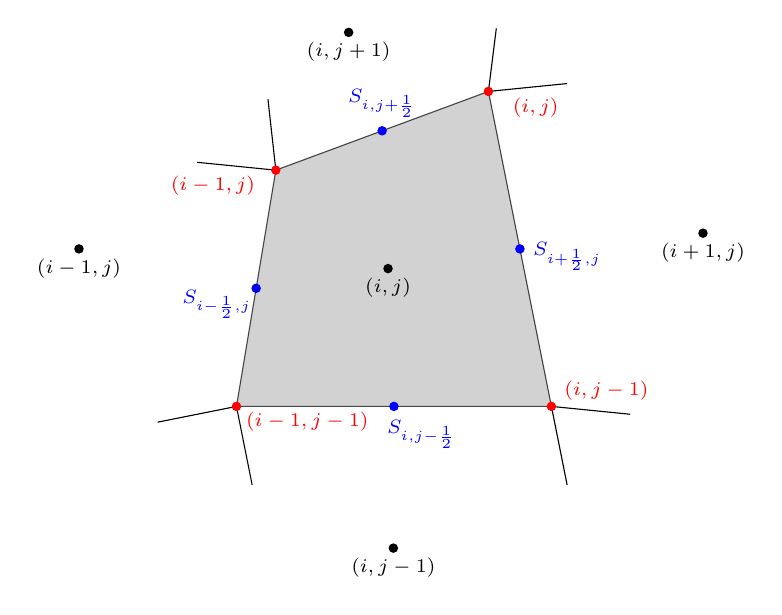
\begin{tikzpicture}
    \draw[fill=lightgray, opacity=0.7] (0,0) -- (4,0) -- (3.2,4) -- (0.5,3) -- (0,0);


    \draw (0,0) -- (-1,-0.2);\draw (0,0) -- (0.2,-1.);
    \draw (4,0) -- (5,-0.1); \draw (4,0) -- (4.2,-1.);
    \draw (3.2,4) -- (4.2,4.1); \draw (3.2,4) -- (3.3,4.8);
    \draw (0.5,3) -- (-0.5,3.1); \draw (0.5,3) -- (0.4,3.9);


    %cell centers
    \draw[fill,black] (1.925,1.75) circle (1.5pt);
    \node[below] at (1.925,1.75) {\scriptsize$(i,j)$};
    \draw[fill,black] (5.925,2.2) circle (1.5pt);
    \node[below] at (5.925,2.2) {\scriptsize$(i+1,j)$};
    \draw[fill,black] (-2,2.) circle (1.5pt);
    \node[below] at (-2,2) {\scriptsize$(i-1,j)$};
    \draw[fill,black] (1.425,4.75) circle (1.5pt);
    \node[below] at (1.425,4.75) {\scriptsize$(i,j+1)$};
    \draw[fill,black] (1.9925,-1.8) circle (1.5pt);
    \node[below] at (1.9925,-1.8) {\scriptsize$(i,j-1)$};


    % nodes
    \node at (0.9,-0.2) {\color{red}\scriptsize$(i-1,j-1)$};
    \node at (4.7,0.2) {\color{red}\scriptsize$(i,j-1)$};
    \node at (3.8,3.8) {\color{red}\scriptsize$(i,j)$};
    \node at (-0.3,2.8) {\color{red}\scriptsize$(i-1,j)$};
    \draw[fill,red] (0,0) circle (1.5pt);
    \draw[fill,red] (4,0) circle (1.5pt);
    \draw[fill,red] (3.2,4) circle (1.5pt);
    \draw[fill,red] (0.5,3) circle (1.5pt);

    %faces
    \node at (-0.25,1.3) {\color{blue}\scriptsize$S_{i-\frac{1}{2},j}$};
    \draw[fill,blue] (0.25,1.5) circle (1.5pt);
    \node at (2.35,-0.35) {\color{blue}\scriptsize$S_{i,j-\frac{1}{2}}$};
    \draw[fill,blue] (2,0) circle (1.5pt);
    \node at (4.2,1.9) {\color{blue}\scriptsize$S_{i+\frac{1}{2},j}$};
    \draw[fill,blue] (3.6,2) circle (1.5pt);
    \node at (1.85,3.85) {\color{blue}\scriptsize$S_{i,j+\frac{1}{2}}$};
    \draw[fill,blue] (1.85,3.5) circle (1.5pt);
\end{tikzpicture}
\end{document}